% TeX file "appendix"

% Master thesis 
% Sven Jacobs
% Winter 2022, M.Sc. Economics, Bonn University
% Supervisor: Prof. Dr. Dominik Liebl


\phantomsection 
\addcontentsline{toc}{section}{Appendix} 

\section*{Appendix}

\renewcommand{\thefigure}{A\arabic{figure}}
\setcounter{figure}{0}
\renewcommand{\thetable}{A\arabic{table}}
\setcounter{table}{0}

\subsection*{Appendix 1: Kernels} \label{appendix:kernels}

\renewcommand{\arraystretch}{1.4}	
\begin{table}[h]
	\centering
	\captionabove{Prominent kernel functions}
	\label{tab:kernels}
	\begin{tabular}{l l c}  
		\toprule
		Kernel & Function & Support \\
		\midrule
		Triangular   & $K_\text{T}(u) = 1 - |u|$       & $[-1, 1]$ \\
		Uniform      & $K_\text{U}(u) = 0.5$           & $[-1, 1]$ \\
		Epanechnikov & $K_\text{E}(u) = 0.75(1 - u^2)$ & $[-1, 1]$ \\
		\bottomrule
	\end{tabular}	
\end{table}
\renewcommand{\arraystretch}{1.0}

\begin{figure}[h]
	\centering
	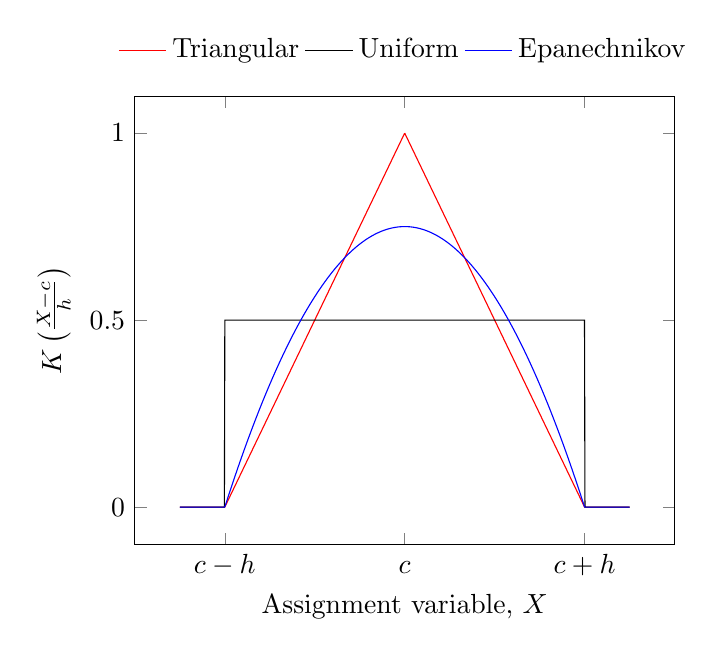
\begin{tikzpicture}
		\begin{axis}
			[
			grid, grid style={white}, 
			samples=1000, 
			domain=-1.25:1.25, 
			xlabel={Assignment variable, $X$}, xtick= {-1, 0, 1},
			xticklabels={$c-h$, \textcolor{white}{h}$c$\textcolor{white}{h}, $c+h$}, 
			ylabel=$K\left(\frac{X-c}{h}\right)$, ytick={0, 0.5, 1},
			legend entries={Triangular, Uniform, Epanechnikov},
			legend style={draw=none}, legend columns=3, legend style={at={(0.5, 1.05)}, anchor=south}
			]
			
			\addplot[red]
			expression {(1 - abs(x)) * (abs(x)<1)};
			
			\addplot[black]
			expression {1/2 * (abs(x)<1)};
			
			\addplot[blue]
			expression {3/4 * (1 - x^2) * (abs(x)<1)};
		\end{axis}
	\end{tikzpicture}
	\caption{Commonly used kernels as given in Table~\ref{tab:kernels}, applied to the RD design}
	\label{fig:kernels}
\end{figure}

\clearpage

\subsection*{Appendix 2: Manipulation of the assignment variable} \label{appendix:manipulation}

\begin{figure}[h]
	\centering
	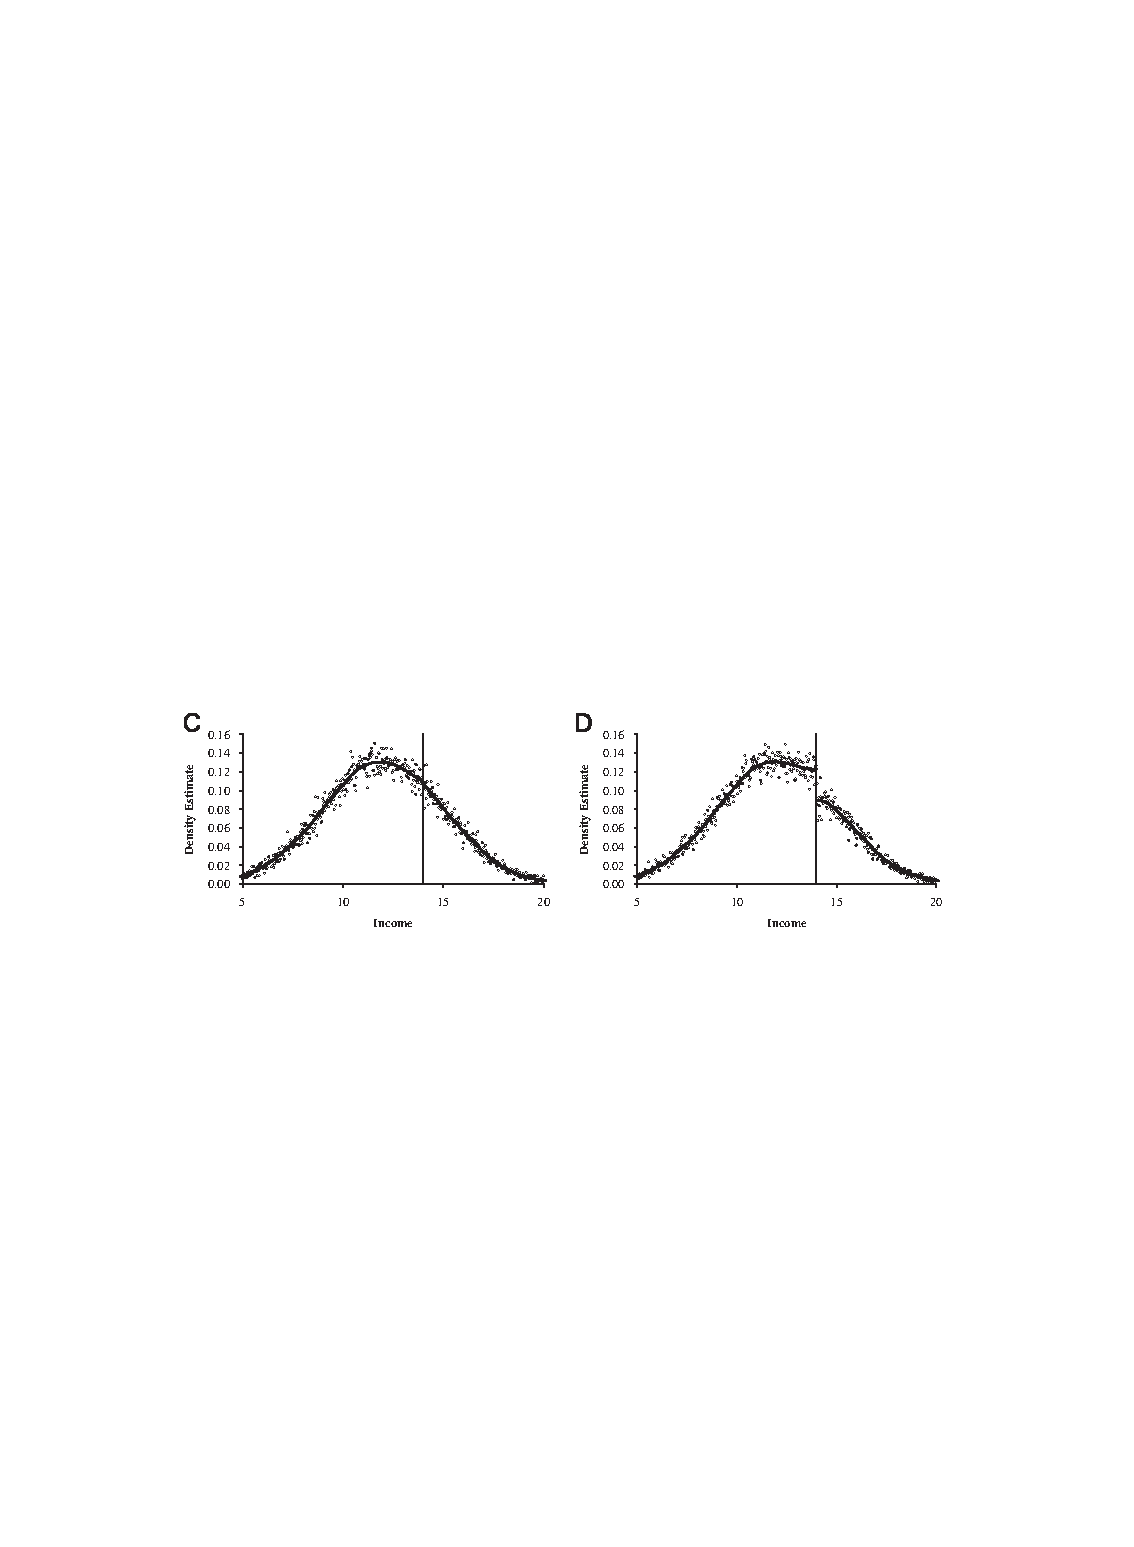
\includegraphics[width=\textwidth]{figure_A02.pdf}
	\caption{Hypothetical example of an income-tested job training program.
			 (C) density of income without manipulation; (D) density of income with manipulation.
		 	 From \textcite[Fig.~2]{McCrary_2008}.}
	\label{fig:McCrary}
\end{figure}

\clearpage

\subsection*{Appendix 3: Application} \label{appendix:application}
\vfill
\begin{figure}[h!]
	\centering
	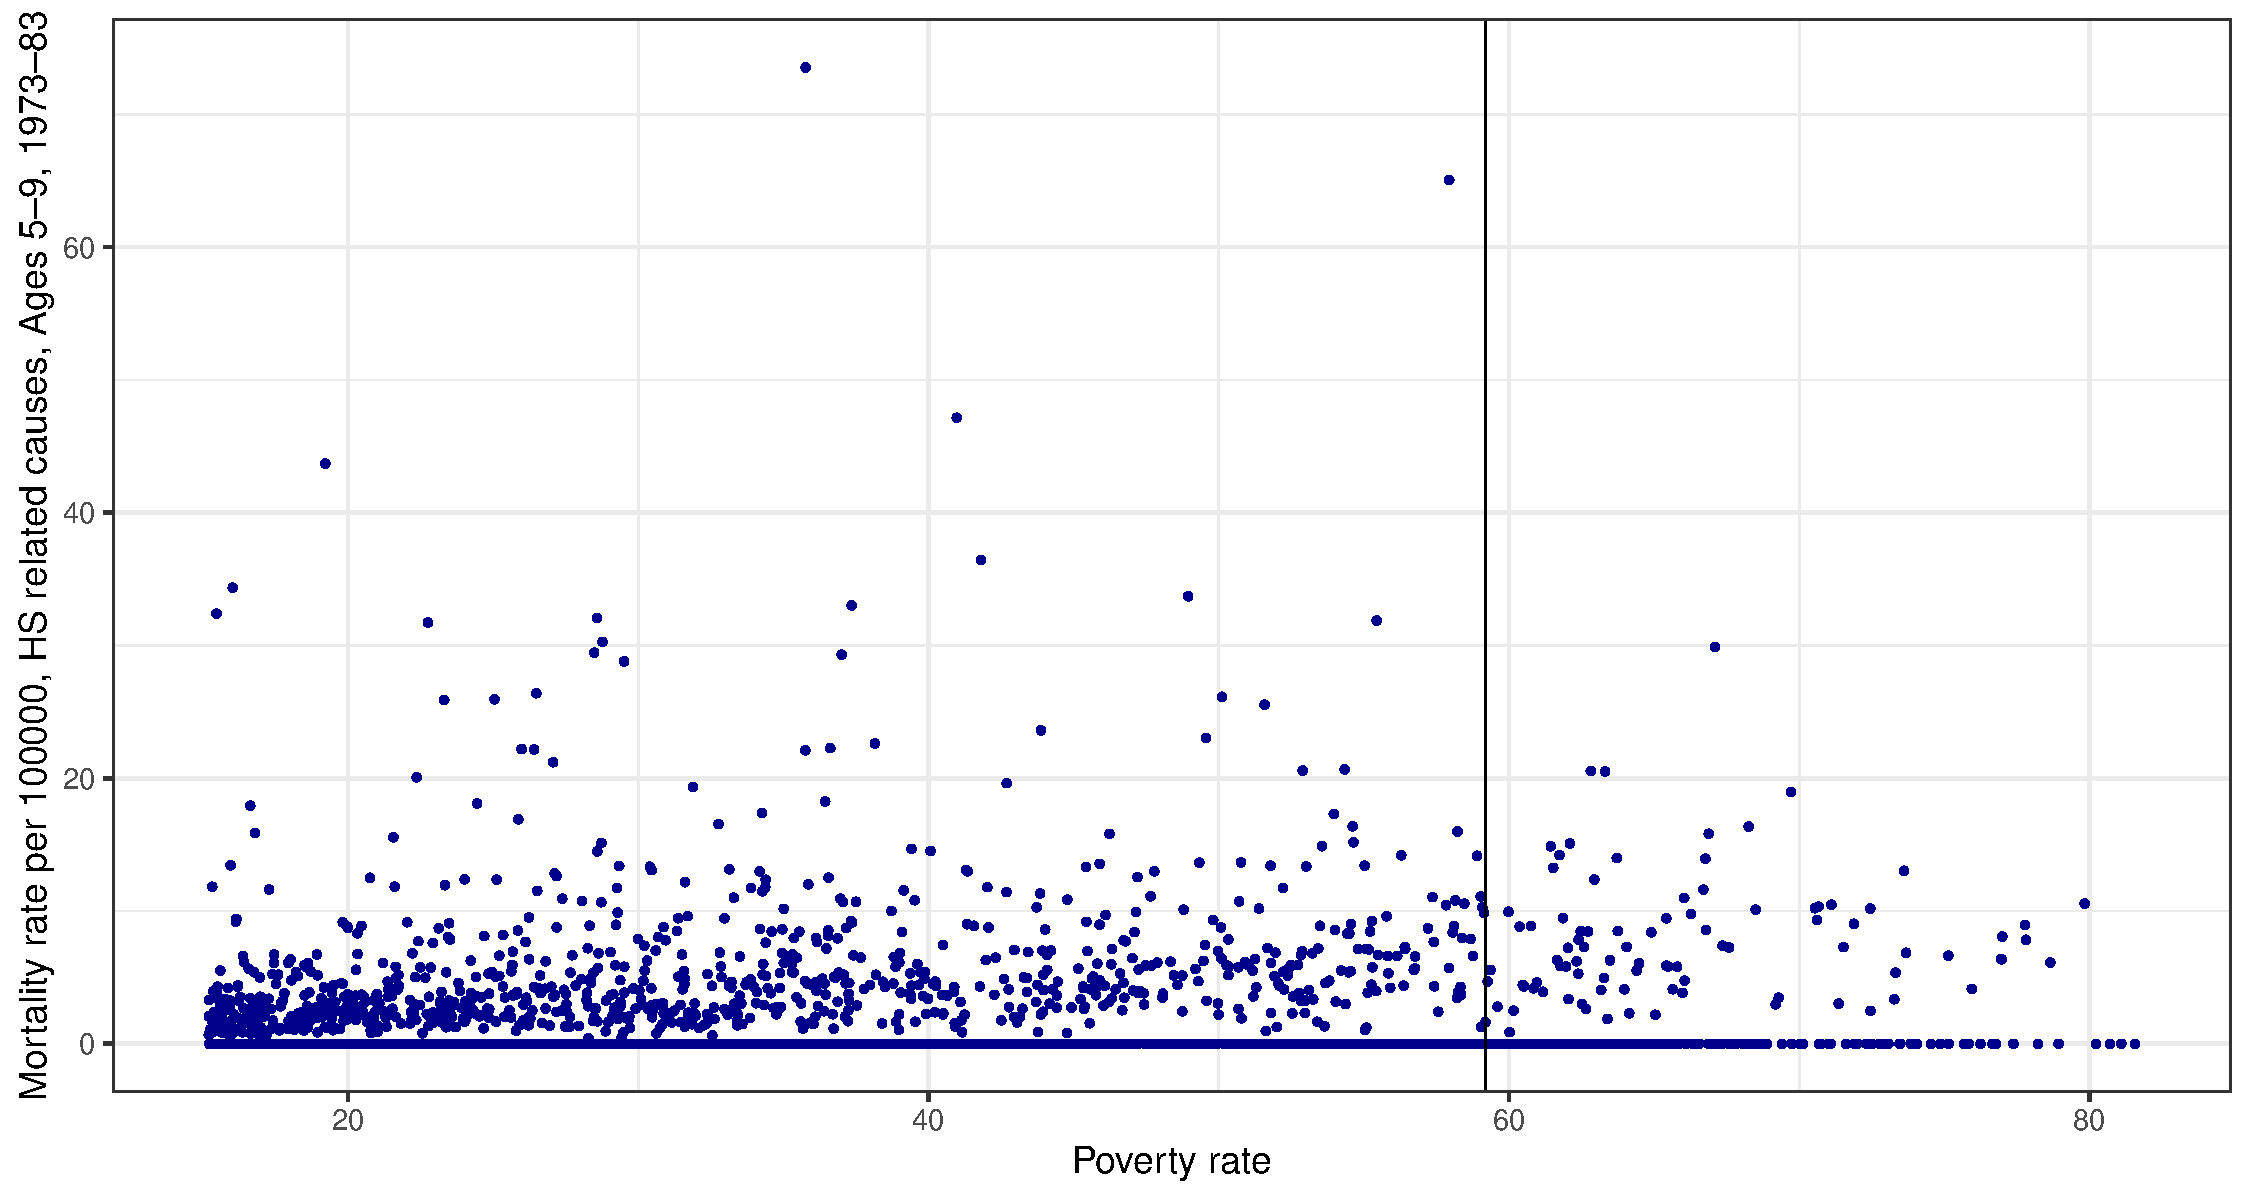
\includegraphics[width=\textwidth]{figure_A03.pdf}
	\caption{Scatter plot of the raw data underlying the Head Start RD analysis.
			 The cutoff of 59.1984 is indicated by the vertical line.}
	\label{fig:scatter}
\end{figure}
\vfill
\begin{figure}[h!]
	\centering
	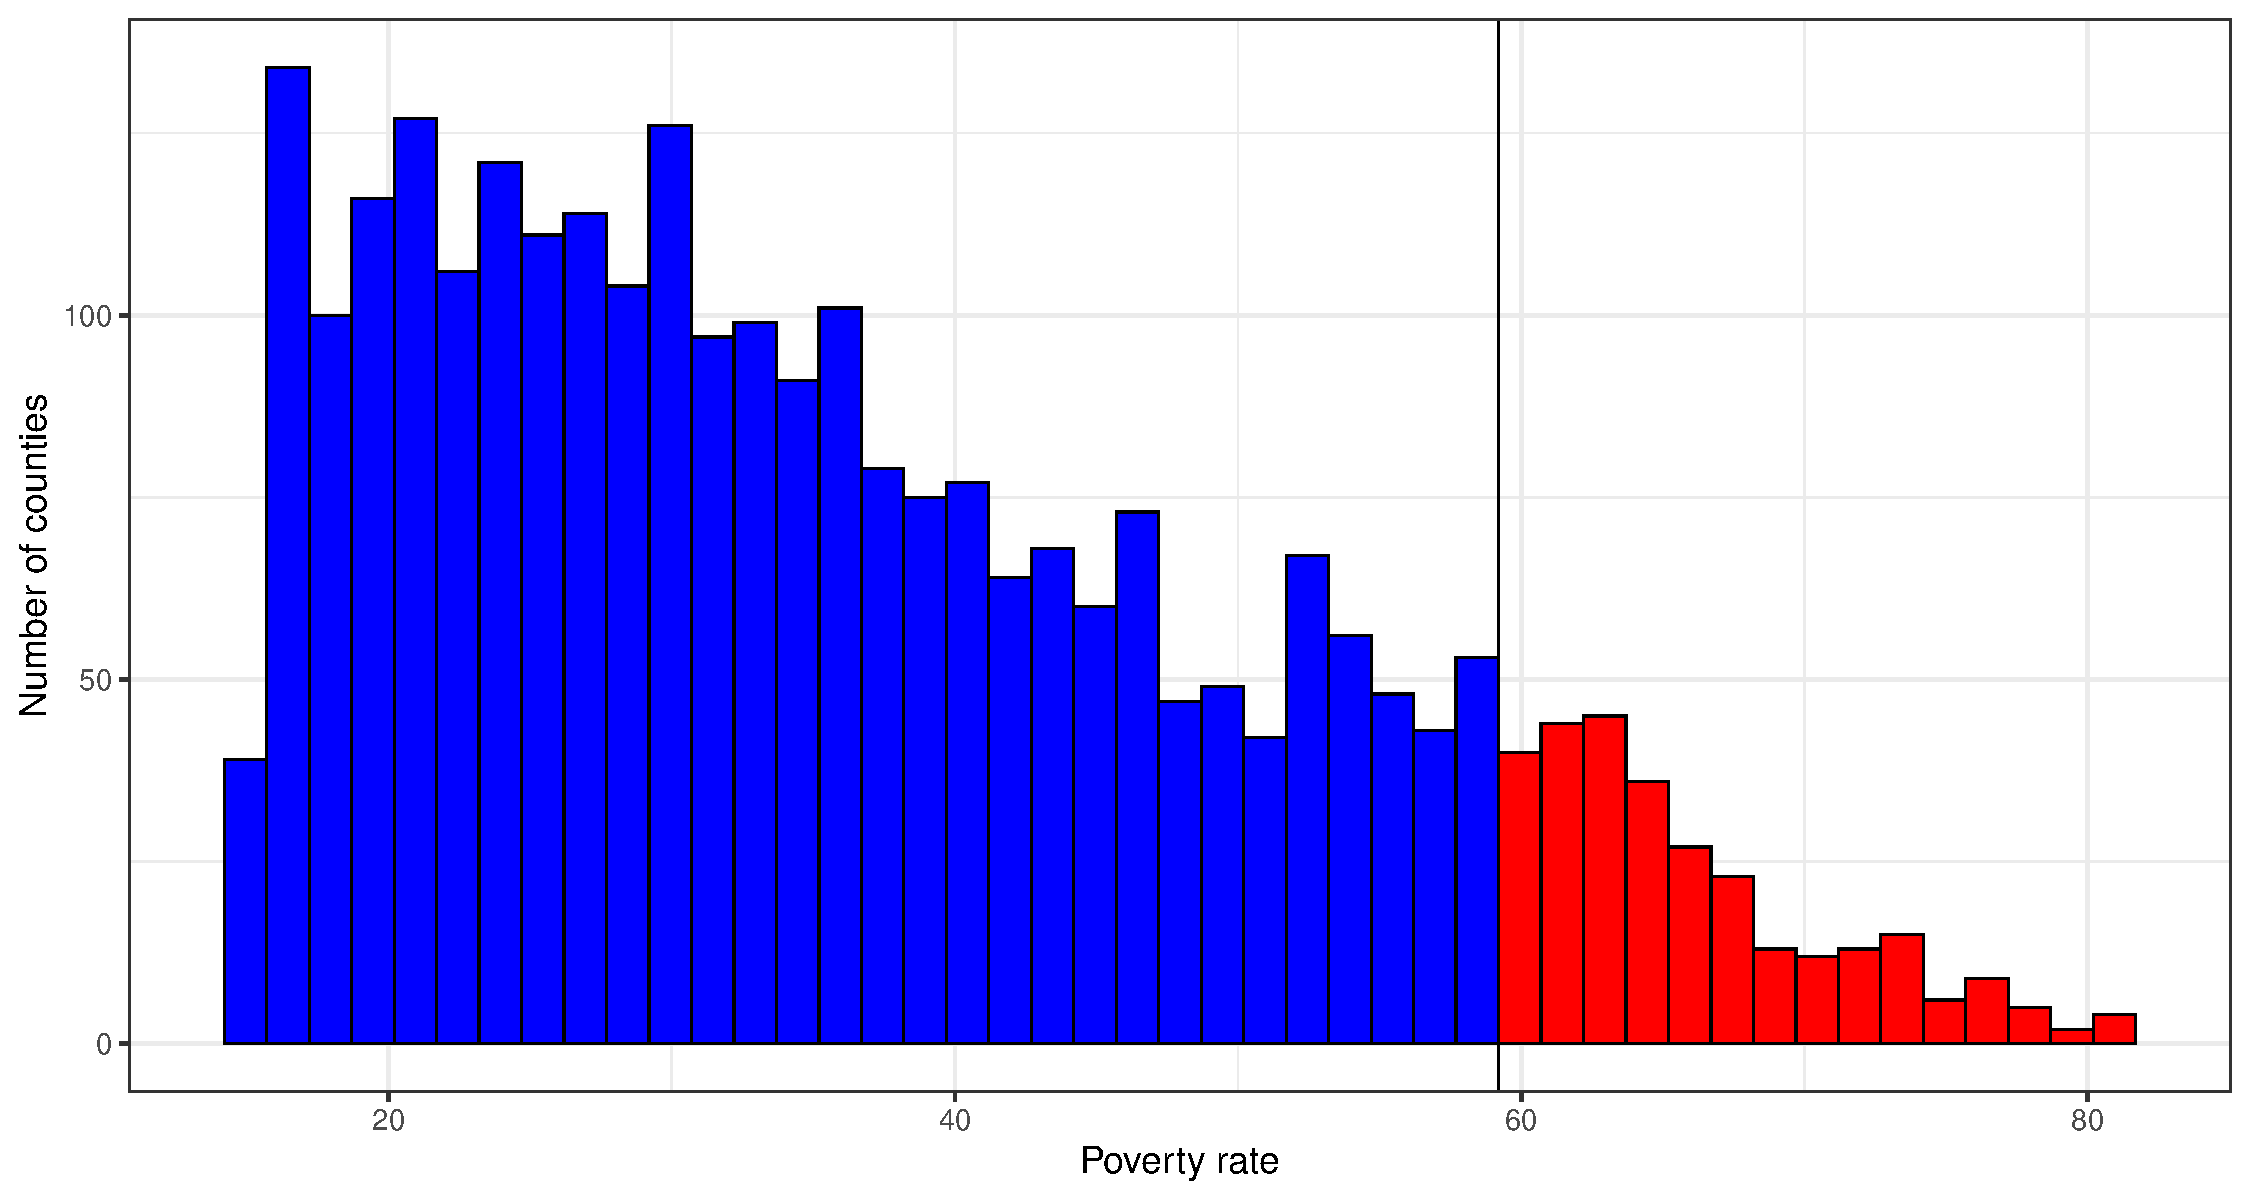
\includegraphics[width=\textwidth]{figure_A04.pdf}
	\caption{Histogram of the poverty rate (assignment variable).
			 The histogram is constructed such that the cutoff (vertical line) constitutes a boundary,
		 	 separating control (blue) and treated (red) counties.}
	\label{fig:histogram}
\end{figure}
\vfill

\clearpage

\vfill
\begin{figure}
	\centering
	\begin{subfigure}[t]{0.49\textwidth}
		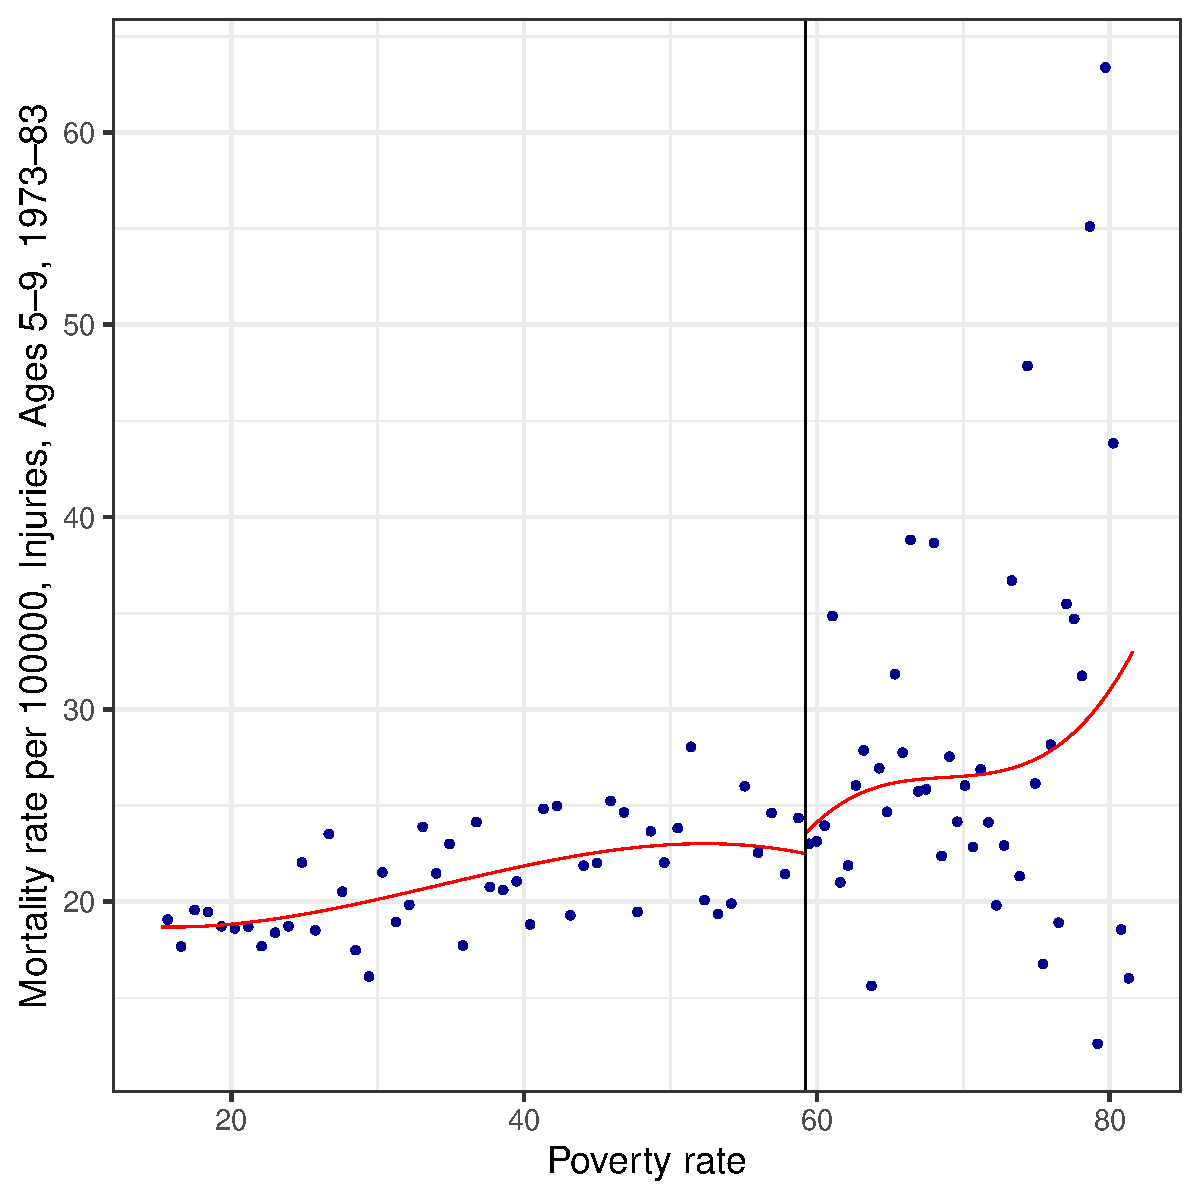
\includegraphics[width=\textwidth]{figure_A05a.pdf}
		\captionsetup{format=hang}
		\caption{Post-treatment placebo outcome injury-related mortality}
		\label{fig:rdplot_injury}
	\end{subfigure}
	\begin{subfigure}[t]{0.49\textwidth}
		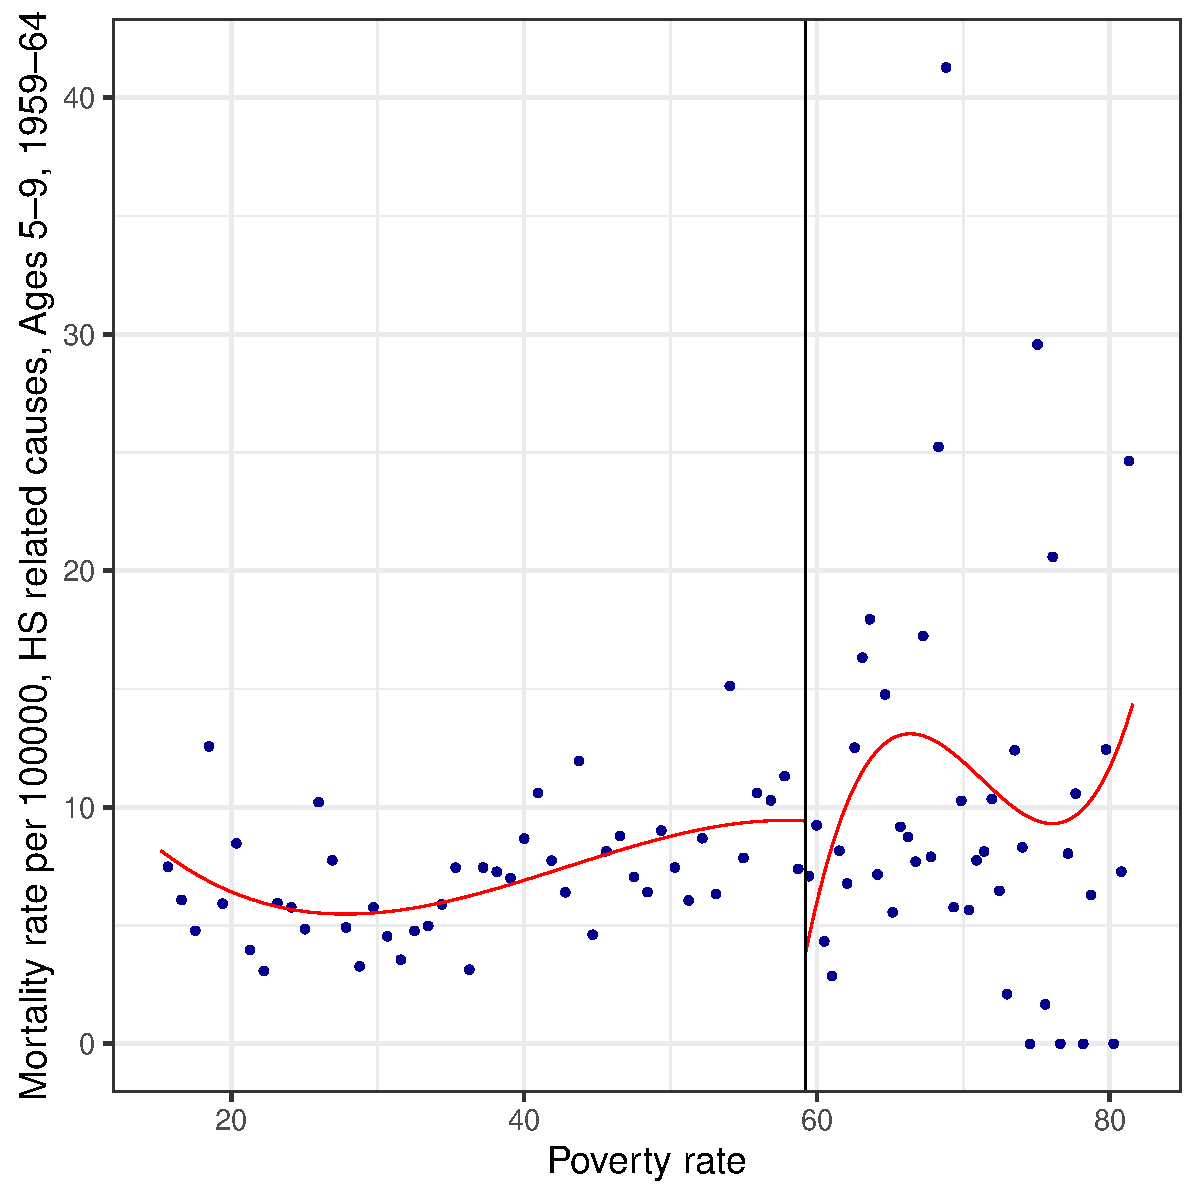
\includegraphics[width=\textwidth]{figure_A05b.pdf}
		\caption{Outcome of interest $(Y)$ before treatment}
		\label{fig:rdplot_Y_pre}
	\end{subfigure}
	\caption{RD plot for two covariates where no treatment effect is expected, to provide evidence for the validity of the RD design.
			 The dots depict the mean within each bin, where the bins are evenly spaced and their number is chosen to mimic variance.
		 	 The solid red lines are third-order polynomial fits for control (left) and treated (right) counties separately.}
	\label{fig:rdplots_cov}
\end{figure}
\vfill
\begin{figure}
	\centering
	\begin{subfigure}[t]{0.49\textwidth}
		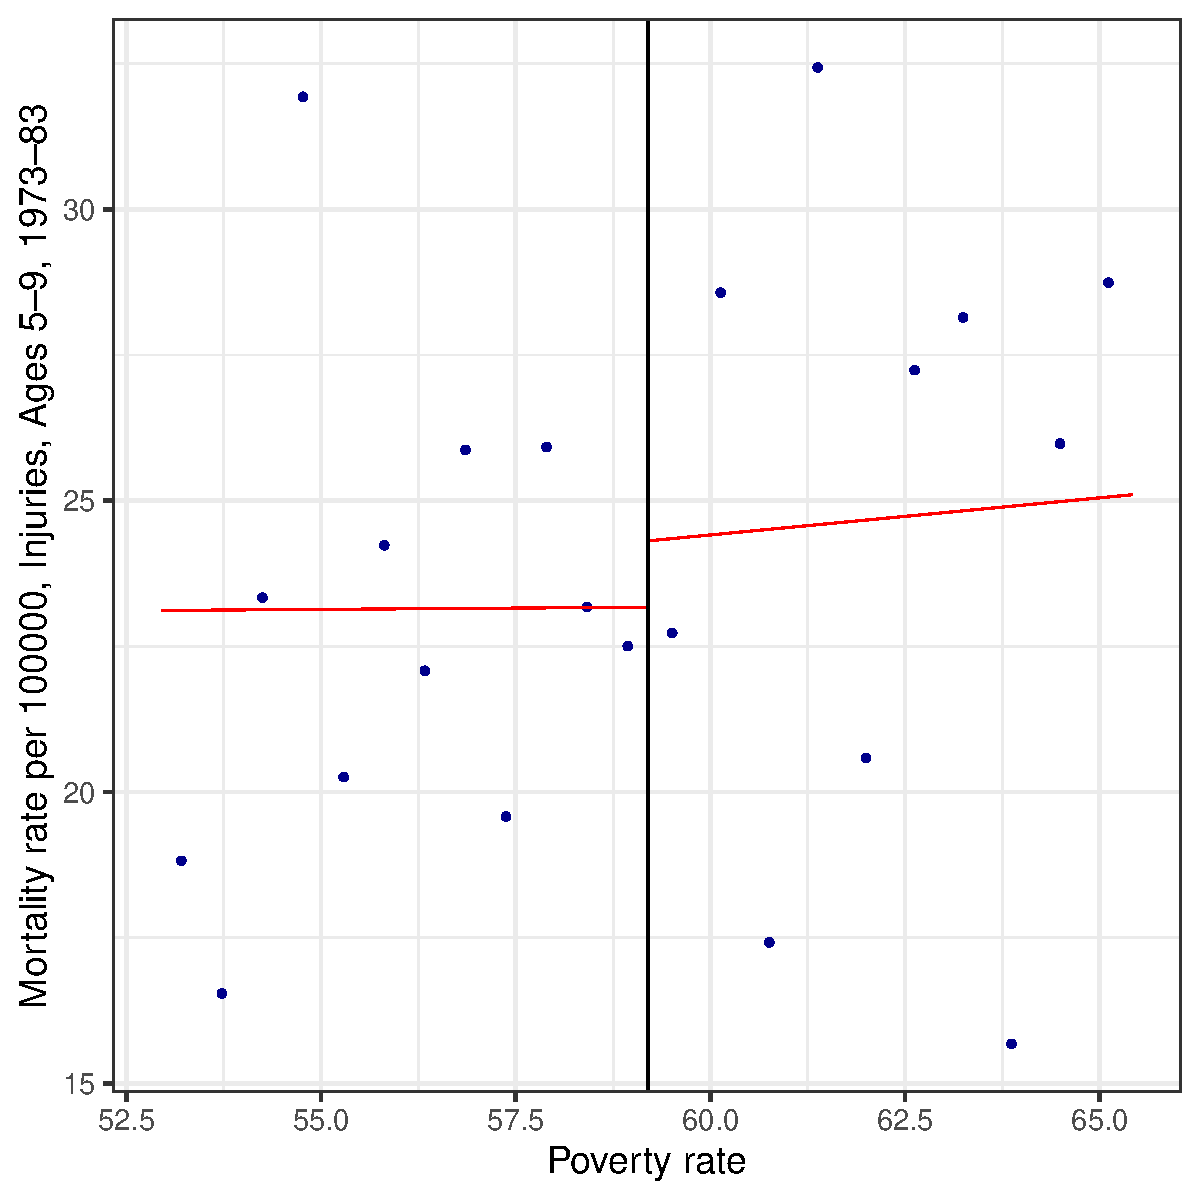
\includegraphics[width=\textwidth]{figure_A06a.pdf}
		\captionsetup{format=hang}
		\caption{Post-treatment placebo outcome injury-related mortality}
		\label{fig:llplot_injury}
	\end{subfigure}
	\begin{subfigure}[t]{0.49\textwidth}
		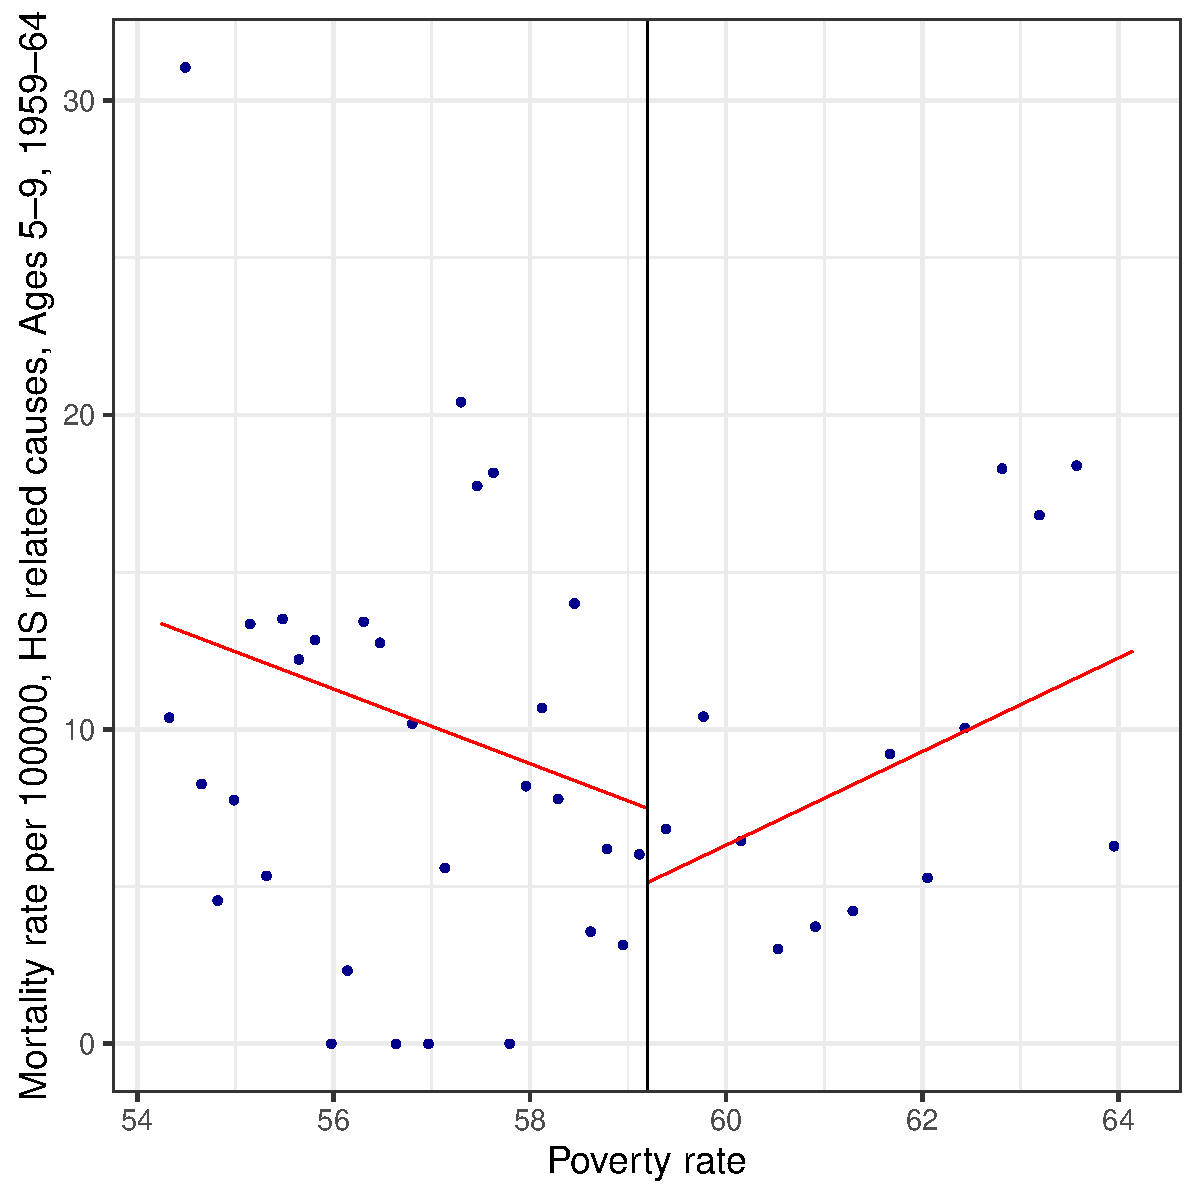
\includegraphics[width=\textwidth]{figure_A06b.pdf}
		\caption{Outcome of interest $(Y)$ before treatment}
		\label{fig:llplot_Y_pre}
	\end{subfigure}
	\caption{As Figure~\ref{fig:rdplots_cov}, but instead of global polynomial fits the local linear fits
			 (triangular kernel, estimated MSE-optimal bandwidth) are displayed.}
	\label{fig:llplots_cov}
\end{figure}
\vfill

\clearpage

\begin{landscape}
\renewcommand{\arraystretch}{1.2}
\begin{table}[p]
	\centering
	\captionabove{RD effect analysis for covariates}
	\label{tab:covariates}
	\begin{tabular}{l r r c c}  
		\toprule
		\multirow{2}[1]{*}{Covariate} & \multirow{2}[1]{*}{$\hat{h}_{\text{MSE}}$} & \multirow{2}[1]{*}{RD estimate} & \multicolumn{2}{c}{RBC inference} \\
		\cmidrule(lr){4-5} 
		& & & 95\% CI & $p$-value \\
		\midrule
		Mortality, Injuries, Ages 5--9, 1973--1983                  & 6.262  & 1.133    & [$-$7.074, 10.120]       & 0.728 \\
		Mortality, All causes, Ages 5--9, 1973--1983                & 6.345  & $-$3.501 & [$-$14.679, 7.371]       & 0.516 \\
		Mortality, Head Start related causes, Ages 25+, 1973--1983  & 8.054  & 2.032    & [$-$12.557, 14.913]      & 0.866 \\
		Mortality, Injuries, Ages 25+, 1973--1983                   & 6.205  & 0.052    & [$-$13.815, 9.693]       & 0.731 \\
		Mortality, Head Start related causes, Ages 5--9, 1959--1964 & 4.963  & $-$2.376 & [$-$7.009, 3.476]        & 0.509 \\
		Census 1960: County population                              & 9.352  & 3084.605 & [$-$5920.470, 11918.011] & 0.510 \\
		Census 1960: \% attending school, Ages 14--17               & 10.083 & 0.557    & [$-$4.335, 5.832]        & 0.773 \\
		Census 1960: \% attending school, Ages 5--34                & 6.194  & 0.906    & [$-$1.345, 3.325]        & 0.406 \\
		Census 1960: \% high school or more, Ages 25+               & 7.651  & 0.621    & [$-$1.490, 2.801]        & 0.549 \\
		Census 1960: Population, Ages 14--17                        & 9.642  & 308.801  & [$-$352.227, 1017.850]   & 0.341 \\
		Census 1960: Population, Ages 5--34                         & 9.703  & 1648.581 & [$-$2977.399, 6400.919]  & 0.474 \\
		Census 1960: Population, Ages 25+                           & 8.312  & 1574.977 & [$-$2894.802, 5741.418]  & 0.518 \\
		Census 1960: \% urban population                            & 8.846  & 2.339    & [$-$5.567, 11.564]       & 0.493 \\
		Census 1960: \% black population                            & 7.166  & 0.793    & [$-$10.237, 11.035]      & 0.941 \\
		\bottomrule \addlinespace[0.25ex]
		\multicolumn{5}{l}{\footnotesize \textit{Note}: Results are based on local linear estimation and the triangular kernel.}
	\end{tabular}	
\end{table}
\renewcommand{\arraystretch}{1.0}
\end{landscape}

\begin{table}[h]
	\centering
	\captionabove{RD effect analysis for placebo cutoffs}
	\label{tab:placebo_cutoffs}
	\begin{tabular}{c c c c c}  
		\toprule
		\multirow{2}[1]{*}{Cutoff} & \multirow{2}[1]{*}{$\hat{h}_{\text{MSE}}$} & \multirow{2}[1]{*}{RD estimate} & \multicolumn{2}{c}{RBC inference} \\
		\cmidrule(lr){4-5} 
		& & & 95\% CI & $p$-value \\
		\midrule
		\multicolumn{5}{c}{Below true cutoff} \\[0.25ex]
		31.463 & 4.595 & \minwd0.032 & [$-$1.142, 1.420]    & 0.831 \\
		40     & 6.114 & \minwd0.015 & [$-$1.494, 2.019]    & 0.769 \\
		50     & 2.340 & \minwd1.894 & [$-$1.689, 6.397]    & 0.254 \\[1ex]
		\multicolumn{5}{c}{True cutoff} \\[0.25ex]
		59.198 & 6.913 & $-$2.389    & [$-$5.426, $-$0.083] & 0.043 \\[1ex]
		\multicolumn{5}{c}{Above true cutoff} \\[0.25ex]
		64.428 & 2.024 & $-$0.490    & [$-$2.802, 2.223]    & 0.821 \\
		70     & 3.054 & $-$1.733    & [$-$15.334, 10.639]  & 0.723 \\
		\bottomrule \addlinespace[0.25ex]
		\multicolumn{5}{l}{\footnotesize \textit{Note}: The median poverty rate for control is 31.463, and for treatment 64.428.} \\[-0.75ex]
		\multicolumn{5}{l}{\footnotesize Results are based on local linear estimation and the triangular kernel.}
	\end{tabular}	
\end{table}

\begin{table}[h]
	\centering
	\captionabove{RD effect analysis for the donut-hole-approach}
	\label{tab:donut_holes}
	\begin{tabular}{c c c c c c c}  
		\toprule
		Radius & \multirow{2}[1]{*}{$\hat{h}_{\text{MSE}}$} & \multirow{2}[1]{*}{RD estimate} & \multicolumn{2}{c}{RBC inference} & \multicolumn{2}{c}{Excluded counties} \\
		\cmidrule(lr){4-5} \cmidrule(lr){6-7} 
		donut hole & & & 95\% CI & $p$-value & Control & Treatment \\
		\midrule
		0.0 & 6.913 & $-$2.389 & [$-$5.426, $-$0.083] & 0.043 & 0  & 0  \\
		0.1 & 6.524 & $-$2.515 & [$-$5.821, $-$0.030] & 0.048 & 3  & 3  \\
		0.2 & 6.371 & $-$2.208 & [$-$5.744, 0.564]    & 0.107 & 6  & 8  \\
		0.3 & 6.407 & $-$1.966 & [$-$5.604, 0.979]    & 0.168 & 9  & 10 \\
		0.4 & 6.438 & $-$2.143 & [$-$6.136, 1.045]    & 0.165 & 12 & 12 \\
		0.5 & 6.468 & $-$2.478 & [$-$7.196, 1.309]    & 0.175 & 18 & 16 \\
		\bottomrule \addlinespace[0.25ex]
		\multicolumn{7}{l}{\footnotesize \textit{Note}: Results are based on local linear estimation and the triangular kernel.}
	\end{tabular}	
\end{table}